
\documentclass[11pt,letterpaper]{article}

% Packages
\usepackage[margin=0.83in]{geometry}
\usepackage[T1]{fontenc}
\usepackage[utf8]{inputenc}
\usepackage{lmodern}
\usepackage{amsmath,amssymb,mathtools}
\usepackage{booktabs,tabularx,array}
\usepackage{xcolor}
\usepackage[most]{tcolorbox}
\usepackage{algorithmicx,algpseudocode}
\usepackage{tikz}
\usetikzlibrary{arrows.meta,positioning,shapes.geometric}
\usepackage{enumitem}
\usepackage{microtype}
\usepackage{fancyhdr}
\usepackage[hidelinks,bookmarks=false]{hyperref}
\usepackage{titlesec}

% Colors
\definecolor{navy}{HTML}{172C45}
\definecolor{ink}{HTML}{222D3C}
\definecolor{muted}{HTML}{617286}
\definecolor{pale}{HTML}{EEF3F8}
\definecolor{lineblue}{HTML}{D5DFEA}
\definecolor{darkgreen}{HTML}{246D56}
\definecolor{softgreen}{HTML}{EFF7F2}
\definecolor{darkred}{HTML}{983D3D}
\definecolor{softred}{HTML}{FBF0EF}

\color{ink}

% Document styling
\hypersetup{
    colorlinks=true,
    linkcolor=navy,
    urlcolor=navy
}

\titleformat{\section}
{\Large\bfseries\color{navy}}
{\thesection.}{0.6em}{}

\titleformat{\subsection}
{\large\bfseries\color{navy}}
{\thesubsection}{0.6em}{}

\titlespacing*{\section}{0pt}{18pt}{8pt}
\titlespacing*{\subsection}{0pt}{12pt}{5pt}

\setlength{\parindent}{0pt}
\setlength{\parskip}{6pt}

\setlist[itemize]{
    leftmargin=1.4em,
    itemsep=2pt,
    topsep=3pt
}

\setlist[enumerate]{
    leftmargin=1.4em,
    itemsep=2pt,
    topsep=3pt
}

% Boxes
\newtcolorbox{idea}[1][]{
    enhanced,
    breakable,
    colback=pale,
    colframe=lineblue,
    boxrule=.6pt,
    arc=2mm,
    left=9pt,
    right=9pt,
    top=7pt,
    bottom=7pt,
    #1
}

\newtcolorbox{goodbox}[1][]{
    enhanced,
    breakable,
    colback=softgreen,
    colframe=darkgreen!30,
    boxrule=.6pt,
    arc=2mm,
    left=9pt,
    right=9pt,
    top=7pt,
    bottom=7pt,
    #1
}

\newtcolorbox{warnbox}[1][]{
    enhanced,
    breakable,
    colback=softred,
    colframe=darkred!28,
    boxrule=.6pt,
    arc=2mm,
    left=9pt,
    right=9pt,
    top=7pt,
    bottom=7pt,
    #1
}

% Mathematical notation
\newcommand{\setminusop}{\mathbin{\backslash}}
\newcommand{\yes}{\mathsf{yes}}
\newcommand{\no}{\mathsf{no}}
\newcommand{\ask}{\mathord{?}}
\newcommand{\Assign}{\operatorname{Assigned}}
\newcommand{\Const}{\operatorname{Const}}
\newcommand{\Consistent}{\operatorname{Consistent}}
\newcommand{\Eval}{\operatorname{Eval}}
\newcommand{\dom}{\operatorname{dom}}
\newcommand{\Prob}{\mathit{Prob}}
\newcommand{\Altern}{\mathit{Altern}}
\newcommand{\Erw}{\mathit{Erw}}
\newcommand{\EXT}{\mathit{EXT}}
\newcommand{\Env}{\mathit{Env}}
\newcommand{\Inst}{\mathit{Inst}}

\newcommand{\key}[1]{
    \textcolor{navy}{\bfseries #1}
}

% Header and footer
\pagestyle{fancy}
\fancyhf{}
\fancyhead[L]{
    \small\color{muted}
    CPSC 433 | Team working notes
}
\fancyhead[R]{
    \small\color{muted}
    OR-tree $\to$ Set-based
}
\fancyfoot[C]{
    \small\color{muted}\thepage
}
\renewcommand{\headrulewidth}{.3pt}
\setlength{\headheight}{14pt}

\begin{document}

% =====================================================
% TITLE
% =====================================================

\begin{center}
    {\LARGE\bfseries\color{navy}
    Scheduling with Two Search Models}\\[6pt]

    {\large
    OR-tree Feasibility
    $\longrightarrow$
    Set-based Optimization}\\[7pt]

    {\small\color{muted}
    CPSC 433 | Team Explanation and Algorithms}
\end{center}

\begin{idea}
\key{The entire idea in two sentences.}

First, we build \emph{one} valid timetable,
assigning classes one at a time in an OR-tree.

Then, starting from that complete timetable,
we use set-based moves and swaps to lower the
soft-constraint penalty without breaking
any hard constraints.
\end{idea}

% =====================================================
\section{Overview of Our Approach}
% =====================================================

Our solution separates the problem into two tasks:

\begin{enumerate}
    \item \textbf{Constraint Satisfaction:}
    Find one valid timetable using OR-tree search.

    \item \textbf{Optimization:}
    Improve that timetable using set-based search.
\end{enumerate}

\begin{center}
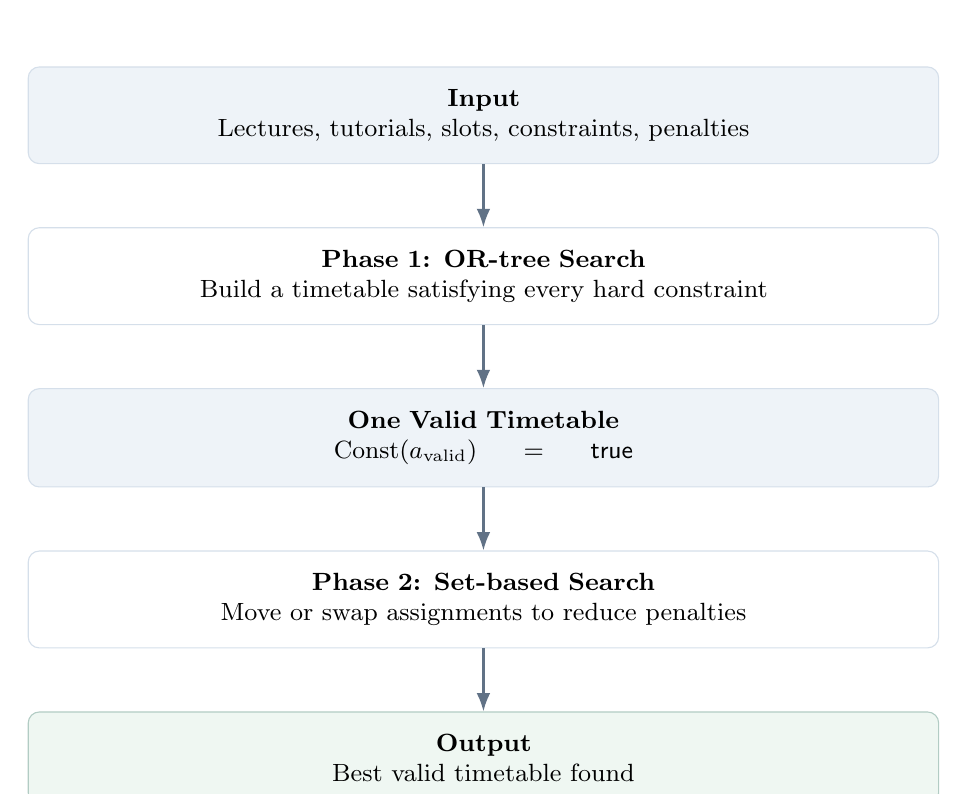
\begin{tikzpicture}[
    >=Latex,
    node distance=8mm,
    every node/.style={font=\small}
]

\node[
    draw=lineblue,
    fill=pale,
    rounded corners=4pt,
    text width=11cm,
    align=center,
    inner sep=8pt
] (start) {
    \textbf{Input}\\
    Lectures, tutorials, slots, constraints, penalties
};

\node[
    draw=lineblue,
    fill=white,
    rounded corners=4pt,
    text width=11cm,
    align=center,
    inner sep=8pt,
    below=of start
] (or) {
    \textbf{Phase 1: OR-tree Search}\\
    Build a timetable satisfying every hard constraint
};

\node[
    draw=lineblue,
    fill=pale,
    rounded corners=4pt,
    text width=11cm,
    align=center,
    inner sep=8pt,
    below=of or
] (handoff) {
    \textbf{One Valid Timetable}\\
    $\Const(a_{\mathrm{valid}})=\mathsf{true}$
};

\node[
    draw=lineblue,
    fill=white,
    rounded corners=4pt,
    text width=11cm,
    align=center,
    inner sep=8pt,
    below=of handoff
] (set) {
    \textbf{Phase 2: Set-based Search}\\
    Move or swap assignments to reduce penalties
};

\node[
    draw=darkgreen!35,
    fill=softgreen,
    rounded corners=4pt,
    text width=11cm,
    align=center,
    inner sep=8pt,
    below=of set
] (end) {
    \textbf{Output}\\
    Best valid timetable found
};

\foreach \a/\b in {
    start/or,
    or/handoff,
    handoff/set,
    set/end}
\draw[->,thick,muted] (\a)--(\b);

\end{tikzpicture}
\end{center}

\begin{warnbox}
\key{Important distinction.}

The OR-tree does not need to generate all valid
timetables. It stops when it finds one complete
valid timetable.

The set-based search then improves that timetable.
It does not construct a new one from scratch.
\end{warnbox}

% =====================================================
\section{Common Definitions}
% =====================================================

Before defining either model, we establish the
scheduling problem.

\begin{tabularx}{\linewidth}{@{}lX@{}}
\toprule
\textbf{Symbol} & \textbf{Meaning}\\
\midrule
$L$ & Set of all lecture sections.\\
$T$ & Set of all tutorials and labs.\\
$X=L\cup T$ & All components requiring scheduling.\\
$S$ & Available weekly time slots.\\
$x\in X$ & An individual lecture or tutorial.\\
$s\in S$ & An individual time slot.\\
$D(x)$ & Allowed time slots for component $x$.\\
$a$ & Assignment of components to slots.\\
$U$ & Set of unscheduled components.\\
$\dom(a)$ & Components already scheduled.\\
$\Consistent(a)$ & Checks whether a partial assignment violates any hard constraint.\\
$\Const(a)$ & Checks whether a complete timetable satisfies all hard constraints.\\
$\Eval(a)$ & Calculates the soft-constraint penalty.\\
\bottomrule
\end{tabularx}

A complete timetable is a function:

\begin{equation}
\boxed{a:X\rightarrow S}
\end{equation}

Every component must be assigned to one
of its allowed time slots:

\begin{equation}
\forall x\in X,\quad a(x)\in D(x)
\end{equation}

Our final optimization objective is:

\begin{equation}
\boxed{
\min_{a:X\rightarrow S}\Eval(a)
}
\end{equation}

Subject to:

\begin{equation}
\boxed{\Const(a)=\mathsf{true}}
\end{equation}

In simple terms, we want a valid timetable
with the smallest possible penalty.

% =====================================================
\section{Worked Scheduling Example}
% =====================================================

We will use four components from CPSC 231.

\begin{tabularx}{\linewidth}{@{}llX@{}}
\toprule
\textbf{Symbol} & \textbf{Component} &
\textbf{Allowed Slots}\\
\midrule
$L_1$ & CPSC 231 LEC 01 &
MWF 9--10\\

$L_2$ & CPSC 231 LEC 02 &
MWF 9--10, 10--11, 11--12\\

$T_1$ & CPSC 231 TUT 01 &
TR 10--11\\

$T_2$ & CPSC 231 TUT 02 &
MW 11--12\\
\bottomrule
\end{tabularx}

For this simplified example, assume:

\begin{itemize}
    \item A time slot supports at most two lectures.
    \item A tutorial slot supports at most one tutorial.
    \item Both tutorials serve both lecture sections.
    \item Tutorials cannot overlap either lecture section.
    \item Scheduling both lecture sections at the same
    time creates a soft penalty of 5.
\end{itemize}

These are assumptions for the worked example,
not the complete project constraints.

Our simplified evaluation function is:

\begin{equation}
\boxed{
\Eval(a)=
5\cdot\mathbf{1}[a(L_1)=a(L_2)]
}
\end{equation}

Where:

\begin{equation}
\mathbf{1}[P]=
\begin{cases}
1 & \text{if proposition }P\text{ is true}\\
0 & \text{otherwise}
\end{cases}
\end{equation}

% =====================================================
\section{Phase 1: OR-tree Search}
% =====================================================

The OR-tree's job is to find a complete
timetable satisfying all hard constraints.

\subsection{Search Model}

Following Lecture 11:

\begin{equation}
\boxed{
A_{\lor}=(S_{\lor},T_{\lor})
}
\end{equation}

Where:

\begin{itemize}
    \item $A_{\lor}$ is the OR-tree search model.
    \item $S_{\lor}$ is the set of OR-tree states.
    \item $T_{\lor}$ is the transition relation.
\end{itemize}

\subsection{Problem Descriptions}

We define an individual scheduling problem:

\begin{equation}
\boxed{
pr=(a,U)
}
\end{equation}

Where:

\begin{itemize}
    \item $pr$ is a problem description.
    \item $a$ is the partial timetable.
    \item $U$ contains unscheduled components.
\end{itemize}

The set of possible problem descriptions is:

\begin{equation}
\boxed{
\Prob=
\left\{
(a,U)\mid
a\text{ is a partial assignment},
\quad
U=X\setminusop\dom(a)
\right\}
}
\end{equation}

Two conditions must always hold:

\begin{equation}
\boxed{
\dom(a)\cap U=\varnothing
}
\end{equation}

\begin{equation}
\boxed{
\dom(a)\cup U=X
}
\end{equation}

These ensure every component is either
scheduled or unscheduled, but never both.

\subsection{OR-tree Nodes}

According to Lecture 11, an OR-tree node is:

\begin{equation}
\boxed{
(pr,sol)
}
\end{equation}

For our scheduling problem:

\begin{equation}
\boxed{
((a,U),sol)
}
\end{equation}

Where:

\begin{equation}
sol\in\{\yes,\ask,\no\}
\end{equation}

The three values mean:

\begin{itemize}
    \item $\yes$: A solution has been found.
    \item $\ask$: The problem is not yet resolved.
    \item $\no$: The problem cannot be completed.
\end{itemize}

Importantly, the search state is the
\textbf{entire OR-tree}, not one individual node.

\begin{equation}
\boxed{
S_{\lor}\subseteq Otree
}
\end{equation}

Here $Otree$ represents the possible OR-tree
structures described in Lecture 11.

\subsection{Alternatives Relation}

The alternatives relation, $\Altern$,
generates different ways to continue scheduling.

Given:

\begin{equation}
pr=(a,U)
\end{equation}

Choose an unscheduled component:

\begin{equation}
x\in U
\end{equation}

Define its currently legal slots:

\begin{equation}
\boxed{
D_a(x)=
\left\{
s\in D(x)\mid
\Consistent(a\cup\{x\mapsto s\})
\right\}
}
\end{equation}

Where:

\begin{itemize}
    \item $D(x)$ is the original set of allowed slots.
    \item $D_a(x)$ contains slots that remain legal
    under the existing partial timetable.
    \item $\Consistent$ checks hard constraints
    involving assignments made so far.
\end{itemize}

For every candidate slot $s_i\in D_a(x)$,
create a new problem:

\begin{equation}
\boxed{
pr_i=
\left(
a\cup\{x\mapsto s_i\},
U\setminusop\{x\}
\right)
}
\end{equation}

If there are $k$ legal slots:

\begin{equation}
\boxed{
\Altern(pr,pr_1,\ldots,pr_k)
}
\end{equation}

Here $k=|D_a(x)|$.

Each alternative assigns one more component.

\subsection{How the Assignment Grows}

At each successful assignment:

\begin{equation}
\boxed{
a_{i+1}=
a_i\cup\{x_i\mapsto s_i\}
}
\end{equation}

\begin{equation}
\boxed{
U_{i+1}=
U_i\setminusop\{x_i\}
}
\end{equation}

Where:

\begin{itemize}
    \item $i$ is the current step.
    \item $x_i$ is the selected component.
    \item $s_i$ is the selected time slot.
\end{itemize}

Therefore:

\begin{equation}
|\dom(a_{i+1})|=|\dom(a_i)|+1
\end{equation}

\begin{equation}
|U_{i+1}|=|U_i|-1
\end{equation}

\subsection{Solved and Unsolvable Problems}

A scheduling problem is solved when:

\begin{equation}
\boxed{
Solved(pr)
\iff
U=\varnothing
\land
\Const(a)=\mathsf{true}
}
\end{equation}

One sufficient condition for an
unsolvable problem is:

\begin{equation}
\boxed{
\exists x\in U:
D_a(x)=\varnothing
}
\end{equation}

This means an unscheduled component
has no legal time slot remaining.

A problem can also be unsolvable when all
of its alternatives have been exhausted.

\subsection{OR-tree Transitions}

Lecture 11 defines transitions using
the extension relation $\Erw_{\lor}$.

\begin{equation}
\boxed{
T_{\lor}=
\left\{
(q,q')\mid
\Erw_{\lor}(q,q')
\text{ or }
\Erw_{\lor}^{*}(q,q')
\right\}
}
\end{equation}

Where $q$ and $q'$ represent entire tree states.

The main extension cases are:

\textbf{Rule 1: Solved Leaf}

\begin{equation}
(pr,\ask)
\longrightarrow
(pr,\yes)
\end{equation}

\textbf{Rule 2: Unsolvable Leaf}

\begin{equation}
(pr,\ask)
\longrightarrow
(pr,\no)
\end{equation}

\textbf{Rule 3: Expand a Leaf}

\begin{equation}
\boxed{
(pr,\ask)
\longrightarrow
(pr,\ask,
(pr_1,\ask),\ldots,(pr_k,\ask))
}
\end{equation}

The extension rules may also be applied
to leaves deeper in the search tree.

\begin{idea}
\key{Why we do not need backtracking.}

If a branch fails, we mark that node
$\no$ and select another unfinished
leaf from the OR-tree.

We do not need an explicit operation
that undoes an earlier tree transition.
\end{idea}

% =====================================================
\section{OR-tree Search Process}
% =====================================================

Following the lecture:

\begin{equation}
\boxed{
P_{\lor}=
(A_{\lor},\Env_{\lor},K_{\lor})
}
\end{equation}

Where:

\begin{itemize}
    \item $P_{\lor}$ is the search process.
    \item $A_{\lor}$ is the search model.
    \item $\Env_{\lor}$ stores scheduling information.
    \item $K_{\lor}$ is the search control.
\end{itemize}

\subsection{Our Search Control}

We propose two main techniques.

\textbf{1. Depth-first leaf selection}

Explore one branch deeply before
selecting a different branch.

\textbf{2. Minimum Remaining Values (MRV)}

Choose the unscheduled component
with the fewest currently legal slots:

\begin{equation}
\boxed{
x^*=
\arg\min_{x\in U}|D_a(x)|
}
\end{equation}

Where $x^*$ is the chosen component.

For this initial design, we order slot
choices by time and explore the earliest
legal slot first.

We are deliberately not using
forward checking in this version.

\subsection{Search Instance}

Following Lecture 11:

\begin{equation}
\boxed{
\Inst_{\lor}=
(q_0,G_{\lor})
}
\end{equation}

Where:

\begin{itemize}
    \item $q_0$ is the initial OR-tree state.
    \item $G_{\lor}$ is the goal condition.
\end{itemize}

Initially:

\begin{equation}
\boxed{
a_0=\varnothing
}
\end{equation}

\begin{equation}
\boxed{
U_0=X
}
\end{equation}

\begin{equation}
\boxed{
pr_0=(a_0,U_0)
}
\end{equation}

\begin{equation}
\boxed{
q_0=(pr_0,\ask)
}
\end{equation}

The search terminates when a solved
branch is found, or all alternatives
have been exhausted.

The outcome is:

\begin{equation}
\boxed{
Outcome_{\lor}(q)=
\begin{cases}
a_{\mathrm{valid}} &
\text{if a solved branch exists}\\
\mathsf{FAILURE} &
\text{if every alternative fails}
\end{cases}
}
\end{equation}

% =====================================================
\section{Algorithm 1: OR-tree Feasibility Search}
% =====================================================

\begin{idea}
\begin{algorithmic}[1]

\Require Components $X$, domains $D$,
hard constraints $\Consistent$

\Ensure One valid timetable or FAILURE

\State $q\gets((\varnothing,X),\ask)$

\While{the tree $q$ contains an unresolved leaf}

    \State $v\gets$ deepest unresolved leaf of $q$

    \State $(a,U)\gets$
    problem description stored at $v$

    \If{$U=\varnothing$}
        \If{$\Const(a)=\mathsf{true}$}
            \State Mark $v$ as $\yes$
            \State \Return $a$
        \Else
            \State Mark $v$ as $\no$
            \State \textbf{continue}
        \EndIf
    \EndIf

    \State $x\gets
    \arg\min_{y\in U}|D_a(y)|$

    \State $C\gets
    \{s\in D(x):
    \Consistent(a\cup\{x\mapsto s\})\}$

    \If{$C=\varnothing$}

        \State Mark $v$ as $\no$

    \Else

        \State Order $C$ by slot time

        \ForAll{$s\in C$}

            \State $a'\gets
            a\cup\{x\mapsto s\}$

            \State $U'\gets
            U\setminusop\{x\}$

            \State Add child
            $((a',U'),\ask)$ to $v$

        \EndFor

    \EndIf

\EndWhile

\State \Return $\mathsf{FAILURE}$

\end{algorithmic}
\end{idea}

The algorithm operates on the OR-tree.
When one alternative fails, another
unfinished leaf can be selected.

No separate backtracking operation
is needed.

% =====================================================
\section{Worked OR-tree Derivation}
% =====================================================

For readability, define:

\begin{align*}
M9 &= \text{MWF 9--10}\\
M10 &= \text{MWF 10--11}\\
M11 &= \text{MWF 11--12}\\
R10 &= \text{TR 10--11}\\
W11 &= \text{MW 11--12}
\end{align*}

\subsection{Initial Problem}

\begin{equation}
a_0=\varnothing
\end{equation}

\begin{equation}
U_0=\{L_1,L_2,T_1,T_2\}
\end{equation}

\subsection{Step 1}

Assign LEC 01 to MWF 9--10.

\begin{equation}
a_1=\{L_1\mapsto M9\}
\end{equation}

\begin{equation}
U_1=\{L_2,T_1,T_2\}
\end{equation}

\subsection{Step 2}

Assign TUT 01 to TR 10--11.

\begin{equation}
a_2=a_1\cup\{T_1\mapsto R10\}
\end{equation}

\begin{equation}
U_2=\{L_2,T_2\}
\end{equation}

\subsection{Step 3}

Assign TUT 02 to MW 11--12.

\begin{equation}
a_3=a_2\cup\{T_2\mapsto W11\}
\end{equation}

\begin{equation}
U_3=\{L_2\}
\end{equation}

\subsection{Step 4}

Only LEC 02 remains unscheduled.

Its original domain is:

\begin{equation}
D(L_2)=\{M9,M10,M11\}
\end{equation}

However:

\begin{equation}
\boxed{
D_{a_3}(L_2)=\{M9,M10\}
}
\end{equation}

MWF 11--12 is excluded because it
overlaps TUT 02 on Monday and Wednesday.

Suppose the OR-tree tries MWF 9--10 first.

\begin{equation}
a_4=a_3\cup\{L_2\mapsto M9\}
\end{equation}

\begin{equation}
\boxed{
U_4=\varnothing
}
\end{equation}

Every component has now been assigned.

\begin{equation}
\boxed{
\Const(a_4)=\mathsf{true}
}
\end{equation}

The leaf is marked:

\begin{equation}
(pr_4,\ask)\rightarrow(pr_4,\yes)
\end{equation}

\begin{goodbox}
\key{End of Phase 1}

The OR-tree returns one valid timetable:

\begin{center}
\begin{tabular}{ll}
LEC 01 & MWF 9--10\\
LEC 02 & MWF 9--10\\
TUT 01 & TR 10--11\\
TUT 02 & MW 11--12
\end{tabular}
\end{center}

Its penalty is:

\[
\boxed{\Eval(a_4)=5}
\]

The two lecture sections share the same time.

This is allowed by our assumed hard constraints,
but creates a soft-constraint penalty.
\end{goodbox}

% =====================================================
\section{Phase 2: Set-based Search}
% =====================================================

Now we already have a valid timetable.

Our goal is to improve its soft-constraint
penalty while keeping it valid.

\subsection{Search Model}

Following Lecture 06:

\begin{equation}
\boxed{
A_{set}=(S_{set},T_{set})
}
\end{equation}

Where:

\begin{itemize}
    \item $A_{set}$ is the set-based search model.
    \item $S_{set}$ is the set of possible states.
    \item $T_{set}$ is the transition relation.
\end{itemize}

\subsection{Facts}

Set-based search represents knowledge
as a set of facts.

We define:

\begin{equation}
\boxed{
F=
\left\{
\Assign(x,s)
\mid
x\in X,\ s\in D(x)
\right\}
}
\end{equation}

Here:

\begin{equation}
\Assign(x,s)
\end{equation}

means component $x$ has been assigned
to time slot $s$.

For example:

\begin{equation}
\Assign(L_1,M9)
\end{equation}

means CPSC 231 LEC 01 is assigned
to MWF 9--10.

\subsection{States}

The lecture defines:

\begin{equation}
S_{set}\subseteq 2^F
\end{equation}

We define our particular state space as:

\begin{equation}
\boxed{
S_{set}=
\left\{
q\subseteq F
\;\middle|\;
\begin{array}{l}
q\text{ assigns every }x\in X
\text{ exactly once,}\\
\Const(a_q)=\mathsf{true}
\end{array}
\right\}
}
\end{equation}

Where:

\begin{itemize}
    \item $q$ is a set of assignment facts.
    \item $a_q$ is the timetable represented by $q$.
\end{itemize}

Every set-based state represents
a complete, valid timetable.

\subsection{Extension Rules}

Lecture 06 defines extension rules:

\begin{equation}
\boxed{
A\rightarrow B
}
\end{equation}

Where:

\begin{itemize}
    \item $A$ contains facts to remove.
    \item $B$ contains replacement facts.
\end{itemize}

We propose two extension rules.

\textbf{Rule 1: Move}

\begin{equation}
\boxed{
\{\Assign(x,s_1)\}
\rightarrow
\{\Assign(x,s_2)\}
}
\end{equation}

Move component $x$ from $s_1$ to $s_2$.

\textbf{Rule 2: Swap}

\begin{equation}
\boxed{
\begin{aligned}
&
\{\Assign(x,s_1),\Assign(y,s_2)\}\\
&\longrightarrow
\{\Assign(x,s_2),\Assign(y,s_1)\}
\end{aligned}
}
\end{equation}

Swap the time slots assigned to components
$x$ and $y$.

Both rules must preserve every hard constraint.
Preassigned components cannot be moved.

\subsection{Transitions}

Following Lecture 06:

\begin{equation}
\boxed{
q'=(q\setminusop A)\cup B
}
\end{equation}

Where:

\begin{itemize}
    \item $q$ is the current state.
    \item $A$ is the set of removed facts.
    \item $B$ is the set of inserted facts.
    \item $q'$ is the new state.
\end{itemize}

The transition relation is:

\begin{equation}
\boxed{
\begin{aligned}
T_{set}=\{(q,q')\mid\;&
\exists(A\rightarrow B)\in\EXT,\\
&A\subseteq q,\\
&q'=(q\setminusop A)\cup B,\\
&q'\in S_{set}
\}
\end{aligned}
}
\end{equation}

The condition $q'\in S_{set}$ ensures
we never move into an invalid timetable.

% =====================================================
\section{Set-based Search Process}
% =====================================================

Following Lecture 06:

\begin{equation}
\boxed{
P_{set}=
(A_{set},\Env_{set},K_{set})
}
\end{equation}

Where:

\begin{itemize}
    \item $P_{set}$ is the search process.
    \item $A_{set}$ is the search model.
    \item $\Env_{set}$ stores relevant information.
    \item $K_{set}$ selects the next transition.
\end{itemize}

\subsection{Weight Function}

The professor introduces $f_{weight}$
to evaluate possible extension rules.

We define:

\begin{equation}
\boxed{
f_{weight}(A,B,e)=
\Eval\left(a_{(q\setminusop A)\cup B}\right)
}
\end{equation}

Where the environment $e$ includes
the current state $q$ and data required
to evaluate the resulting timetable.

The weight is the soft-constraint
penalty after performing the move.

\textbf{Lower weight means a better timetable.}

\subsection{Tie-breaking Function}

If multiple extension rules produce
the same minimum weight, use:

\begin{equation}
\boxed{
f_{select}
}
\end{equation}

Our initial design selects randomly
among the equally best extensions.

\subsection{Hill-climbing Control}

For simplicity, our first implementation
uses strict hill climbing.

Define the neighborhood:

\begin{equation}
\boxed{
N(q)=
\left\{
q'\in S_{set}
\mid
(q,q')\in T_{set},\ q'\neq q
\right\}
}
\end{equation}

Where $N(q)$ contains all valid timetables
reachable by one move or swap.

Choose the neighbor with the
lowest penalty.

We only perform a move if:

\begin{equation}
\boxed{
\min_{q'\in N(q)}
\Eval(a_{q'})
<
\Eval(a_q)
}
\end{equation}

If there is no improving neighbor,
the algorithm stops.

This is called a \textbf{local optimum}.

It may not be the global optimum.

\subsection{Search Instance}

Following Lecture 06:

\begin{equation}
\boxed{
\Inst_{set}=(q_0,G_{set})
}
\end{equation}

Our initial state is generated
from the OR-tree solution:

\begin{equation}
\boxed{
q_0=
\left\{
\Assign(x,a_{\mathrm{valid}}(x))
\mid
x\in X
\right\}
}
\end{equation}

The search terminates when:

\begin{itemize}
    \item The penalty reaches zero, or
    \item No improving neighbor remains.
\end{itemize}

A practical implementation may also
use a time or iteration limit.

% =====================================================
\section{Algorithm 2: Set-based Optimization}
% =====================================================

\begin{idea}
\begin{algorithmic}[1]

\Require Valid timetable $a_{\mathrm{valid}}$,
allowed slots, hard constraints, $\Eval$

\Ensure Improved valid timetable

\State $q\gets
\{\Assign(x,a_{\mathrm{valid}}(x)):
x\in X\}$

\While{$\Eval(a_q)>0$}

    \State $N\gets
    \{q'\in S_{set}:
    (q,q')\in T_{set},\ q'\neq q\}$

    \If{$N=\varnothing$}
        \State \Return $a_q$
    \EndIf

    \State $m\gets
    \min\{\Eval(a_{q'}):q'\in N\}$

    \If{$m\geq\Eval(a_q)$}
        \State \Return $a_q$
    \EndIf

    \State $B\gets
    \{q'\in N:\Eval(a_{q'})=m\}$

    \State $q\gets f_{select}(B)$

\EndWhile

\State \Return $a_q$

\end{algorithmic}
\end{idea}

For readability, the algorithm above
uses $f_{select}$ to choose a neighboring
state.

In Lecture 06, $f_{select}$ formally
chooses among equally weighted
extension rules that produce those states.

% =====================================================
\section{Worked Set-based Derivation}
% =====================================================

Our OR-tree returned:

\begin{equation}
\begin{aligned}
q_0=\{&
\Assign(L_1,M9),\\
&
\Assign(L_2,M9),\\
&
\Assign(T_1,R10),\\
&
\Assign(T_2,W11)
\}
\end{aligned}
\end{equation}

Its initial penalty is:

\begin{equation}
\boxed{
\Eval(a_{q_0})=5
}
\end{equation}

The optimizer considers moving LEC 02
from MWF 9--10 to MWF 10--11.

Define:

\begin{equation}
A=\{\Assign(L_2,M9)\}
\end{equation}

\begin{equation}
B=\{\Assign(L_2,M10)\}
\end{equation}

Apply the set-based transition:

\begin{equation}
\boxed{
q_1=(q_0\setminusop A)\cup B
}
\end{equation}

The new state becomes:

\begin{equation}
\begin{aligned}
q_1=\{&
\Assign(L_1,M9),\\
&
\Assign(L_2,M10),\\
&
\Assign(T_1,R10),\\
&
\Assign(T_2,W11)
\}
\end{aligned}
\end{equation}

This timetable satisfies all hard constraints.

The two lecture sections now occupy
different time slots.

Therefore:

\begin{equation}
\boxed{
\Eval(a_{q_1})=0
}
\end{equation}

\begin{goodbox}
\key{Final Improvement}

\[
\boxed{
5\longrightarrow0
}
\]

The OR-tree found a valid solution
with penalty 5.

The set-based search changed one
assignment and reduced the penalty to 0.
\end{goodbox}

\subsection{Final Timetable}

\begin{tabularx}{\linewidth}{@{}lXX@{}}
\toprule
\textbf{Component} &
\textbf{OR-tree Output} &
\textbf{Final Timetable}\\
\midrule
CPSC 231 LEC 01 &
MWF 9--10 &
MWF 9--10\\

CPSC 231 LEC 02 &
MWF 9--10 &
\textbf{MWF 10--11}\\

CPSC 231 TUT 01 &
TR 10--11 &
TR 10--11\\

CPSC 231 TUT 02 &
MW 11--12 &
MW 11--12\\
\midrule
Soft penalty &
$5$ &
$\mathbf{0}$\\
\bottomrule
\end{tabularx}

% =====================================================
\section{Strengths and Limitations}
% =====================================================

\subsection{Strengths}

\begin{itemize}
    \item The two models have clearly
    separated responsibilities.

    \item The OR-tree focuses on satisfying
    hard constraints.

    \item Set-based search focuses on
    minimizing soft penalties.

    \item The design closely follows the
    search-model terminology from
    Lectures 06 and 11.

    \item The set-based optimizer always
    maintains a valid timetable.
\end{itemize}

\subsection{Limitations}

\begin{itemize}
    \item OR-tree search can require
    exploring many alternatives.

    \item Storing the OR-tree can consume
    substantial memory.

    \item Hill climbing may get stuck
    at a local optimum.

    \item Single moves and swaps may
    be insufficient for some schedules.

    \item The final timetable is not
    guaranteed to have the globally
    minimum possible penalty.
\end{itemize}

Possible future improvements include:

\begin{itemize}
    \item Forward checking for OR-tree search.
    \item Least Constraining Value slot ordering.
    \item Multi-component assignment moves.
    \item Random restarts.
    \item Simulated annealing.
\end{itemize}

% =====================================================
\section{Three Important Invariants}
% =====================================================

These are conditions that our implementation
should maintain.

\textbf{Invariant 1: OR-tree Partition}

\begin{equation}
\boxed{
\dom(a)\cap U=\varnothing
}
\end{equation}

\begin{equation}
\boxed{
\dom(a)\cup U=X
}
\end{equation}

Every component is either already assigned
or waiting to be assigned.

\textbf{Invariant 2: OR-tree Legality}

Every generated child must satisfy:

\begin{equation}
\boxed{
\Consistent(a)=\mathsf{true}
}
\end{equation}

Each child adds exactly one assignment.

\textbf{Invariant 3: Set-based Validity}

Every state $q\in S_{set}$ represents
a complete valid timetable:

\begin{equation}
\boxed{
\Const(a_q)=\mathsf{true}
}
\end{equation}

All moves and swaps must preserve this property.

% =====================================================
\section*{Final Summary}
% =====================================================

\begin{idea}
\textbf{OR-tree Search}

Start with:

\[
a=\varnothing,\qquad U=X
\]

Choose an unscheduled component,
generate alternative legal assignments,
and grow the search tree.

Stop when:

\[
U=\varnothing
\quad\land\quad
\Const(a)=\mathsf{true}
\]

Return one valid timetable.

\vspace{8pt}

\textbf{Set-based Search}

Convert the valid timetable
into a set of assignment facts:

\[
q=\{\Assign(x,s),\ldots\}
\]

Generate valid moves and swaps,
evaluate their penalties, and
continue improving while possible.

\vspace{8pt}

\textbf{The key distinction}

A valid timetable is not necessarily
an optimal timetable.

The OR-tree finds something that works.

The set-based search tries to make it better.
\end{idea}

\end{document}
